\documentclass[tikz]{standalone}
\usepackage{amsmath}

\tikzset{
    grid/.style={very thin, draw=gray!50},
    brane/.style={fill=gray!40},
    minimal_surface/.style={fill=blue!40}
}

\begin{document}
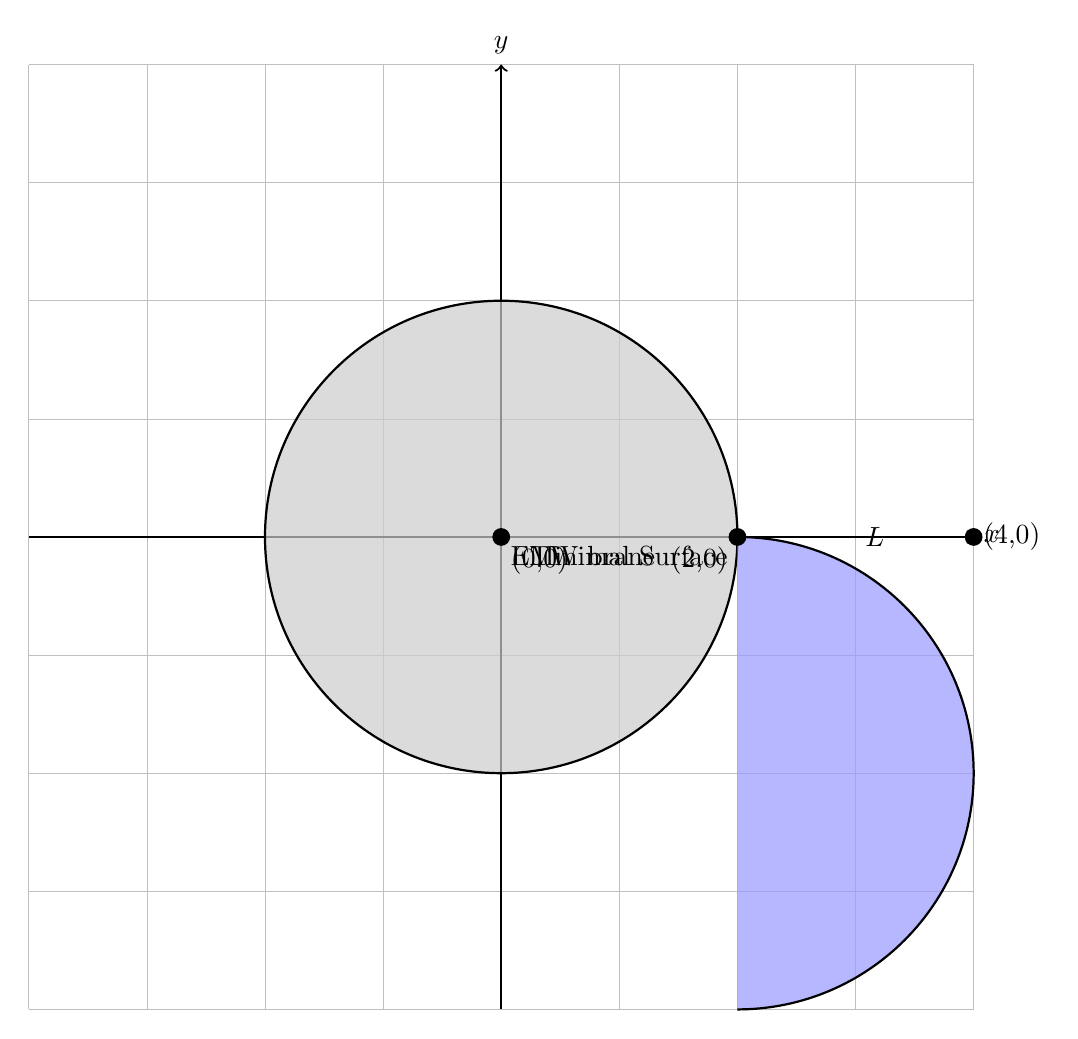
\begin{tikzpicture}[scale=1.5]

% Draw the grid
\draw[grid] (-4,-4) grid (4,4);

% Draw the AdS_3 plane
\draw[thick, ->] (-4,0) -- (4,0) node[right] {$x$};
\draw[thick, ->] (0,-4) -- (0,4) node[above] {$y$};

% Draw the brane
\draw[brane, thick, fill opacity=0.7] (0,0) circle (2cm);
\node at (0,0) [below right] {ETW brane};

% Draw the minimal surface
\draw[minimal_surface, thick, fill opacity=0.7] (2,0) arc[start angle=90, end angle=-90, radius=2];
\node at (2,0) [below left] {Minimal Surface};

% Draw the line L
\draw[dashed, thick] (2,0) -- (4,0);
\node at (3,0) [right] {$L$};

% Draw the intersection points
\filldraw (0,0) circle (2pt) node[below right] {(0,0)};
\filldraw (2,0) circle (2pt) node[below left] {(2,0)};
\filldraw (4,0) circle (2pt) node[right] {(4,0)};

\end{tikzpicture}
\end{document}